
\begin{frame}
    \frametitle{Human Driven - Car following model}
    \begin{columns}
    \begin{column}{0.5\textwidth}
      \begin{figure}
        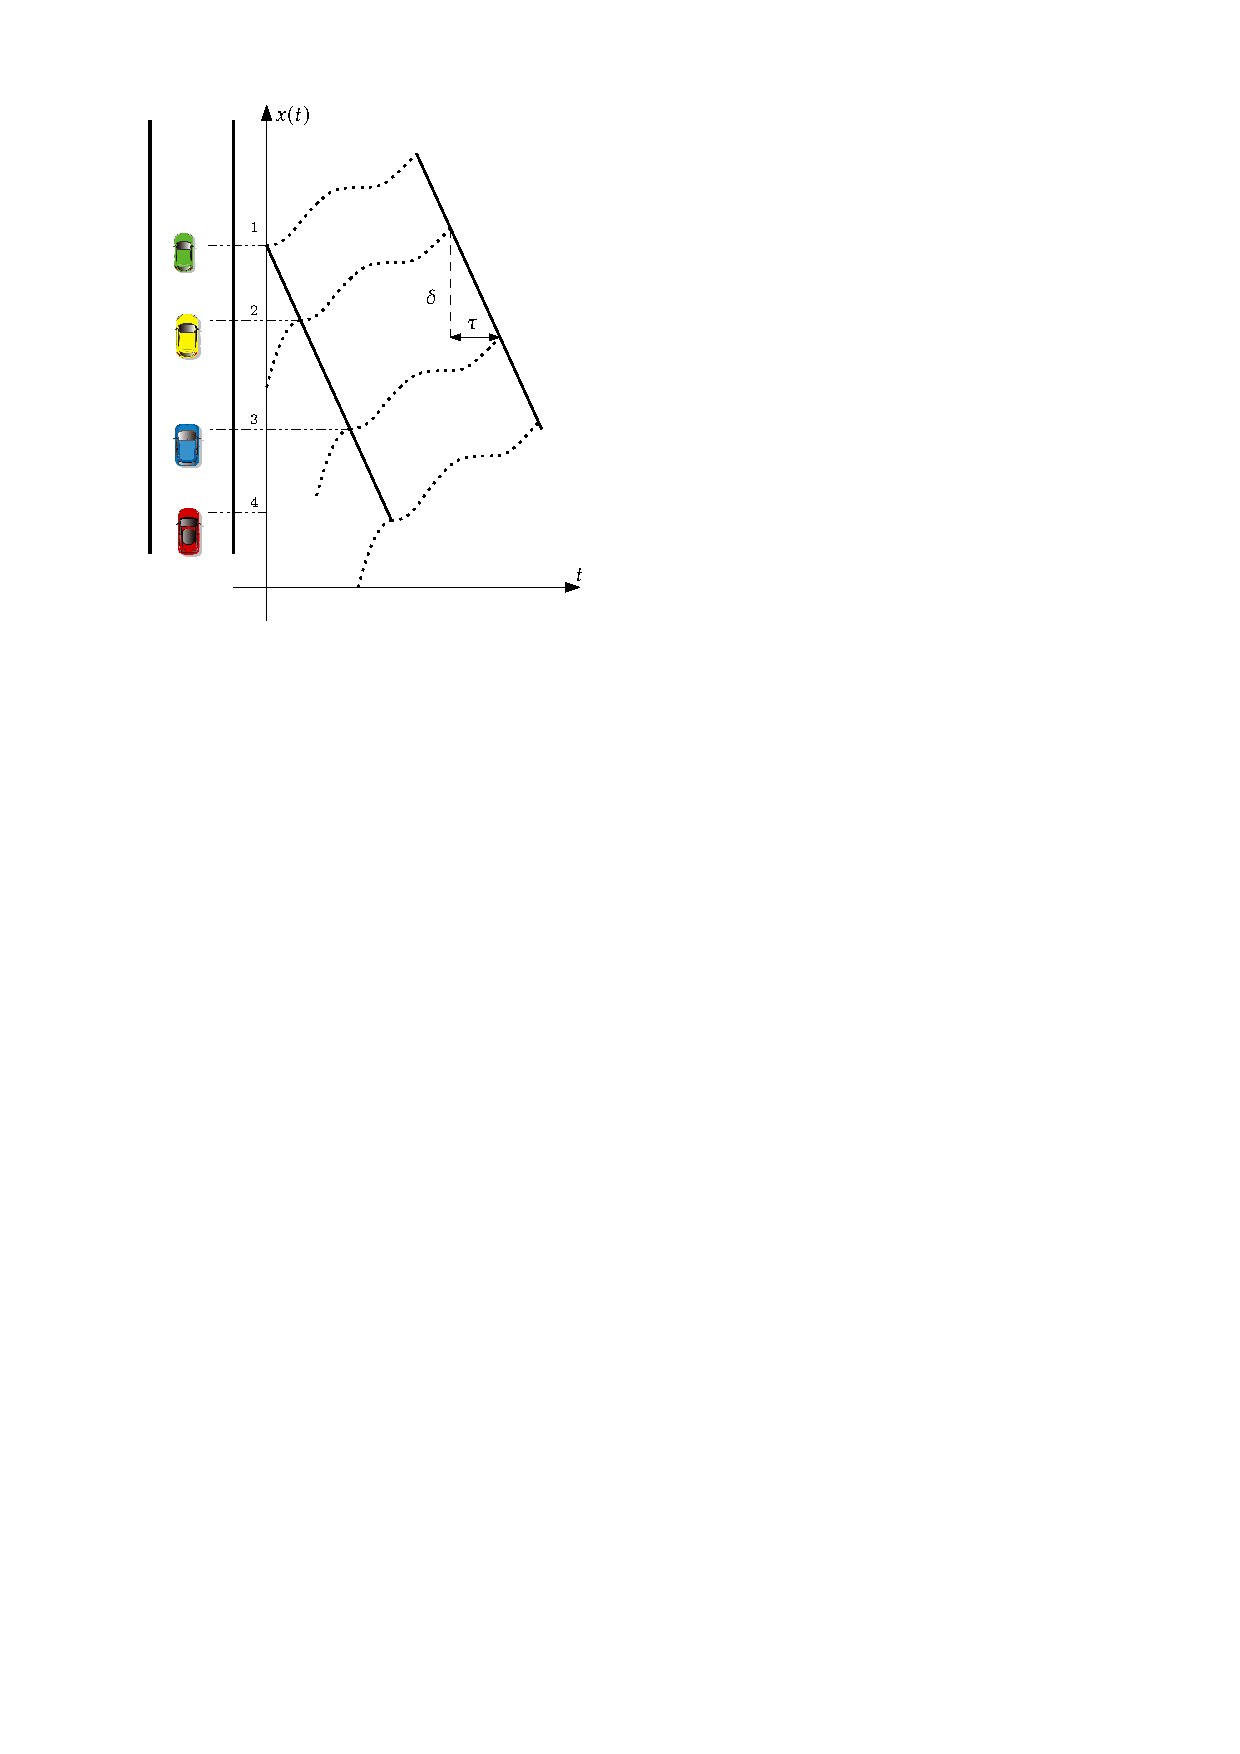
\includegraphics[width=0.8\linewidth]{fig_2_time_space}
      \end{figure}
      \uncover<2-|handout:1>{
      \begin{equation*}
        \scriptsize
        \begin{aligned}
          x_i(t) = \min(x^F_i(t),x^C_i(t))\\
          \begin{cases}
            x^F_{i}(t)= x_i(t-\tau) + u \tau \\
            x^C_{i}(t)= x_{i-1}(t-\tau) - \delta
          \end{cases}
        \end{aligned}
      \end{equation*}
      }
    \end{column}
    \begin{column}{0.7\textwidth}
      \begin{center}
      \uncover<3-|handout:1>{
      \begin{itemize}
      \item Truck properties
        \begin{itemize}
          \item[\(L\)] Vehicle's length 
          \item[\(u\)] Free flow speed 
          \item[\(\kappa_x\)] Maximum density
        \end{itemize}
      % \onslide<2->{Truck properties}
      \item Platoon properties 
        \begin{itemize}
          \item[\(N\)] Number of trucks 
          \item[\(g_t\)] Time gap policy
        \end{itemize}
      % \onslide<3->{Time headway inside the platoon (front to front)}
      \item Time headway: \(h^p = g^t + L/u\)
      \end{itemize}
      }
      \only<2-3|handout:0>{
      \begin{figure}
          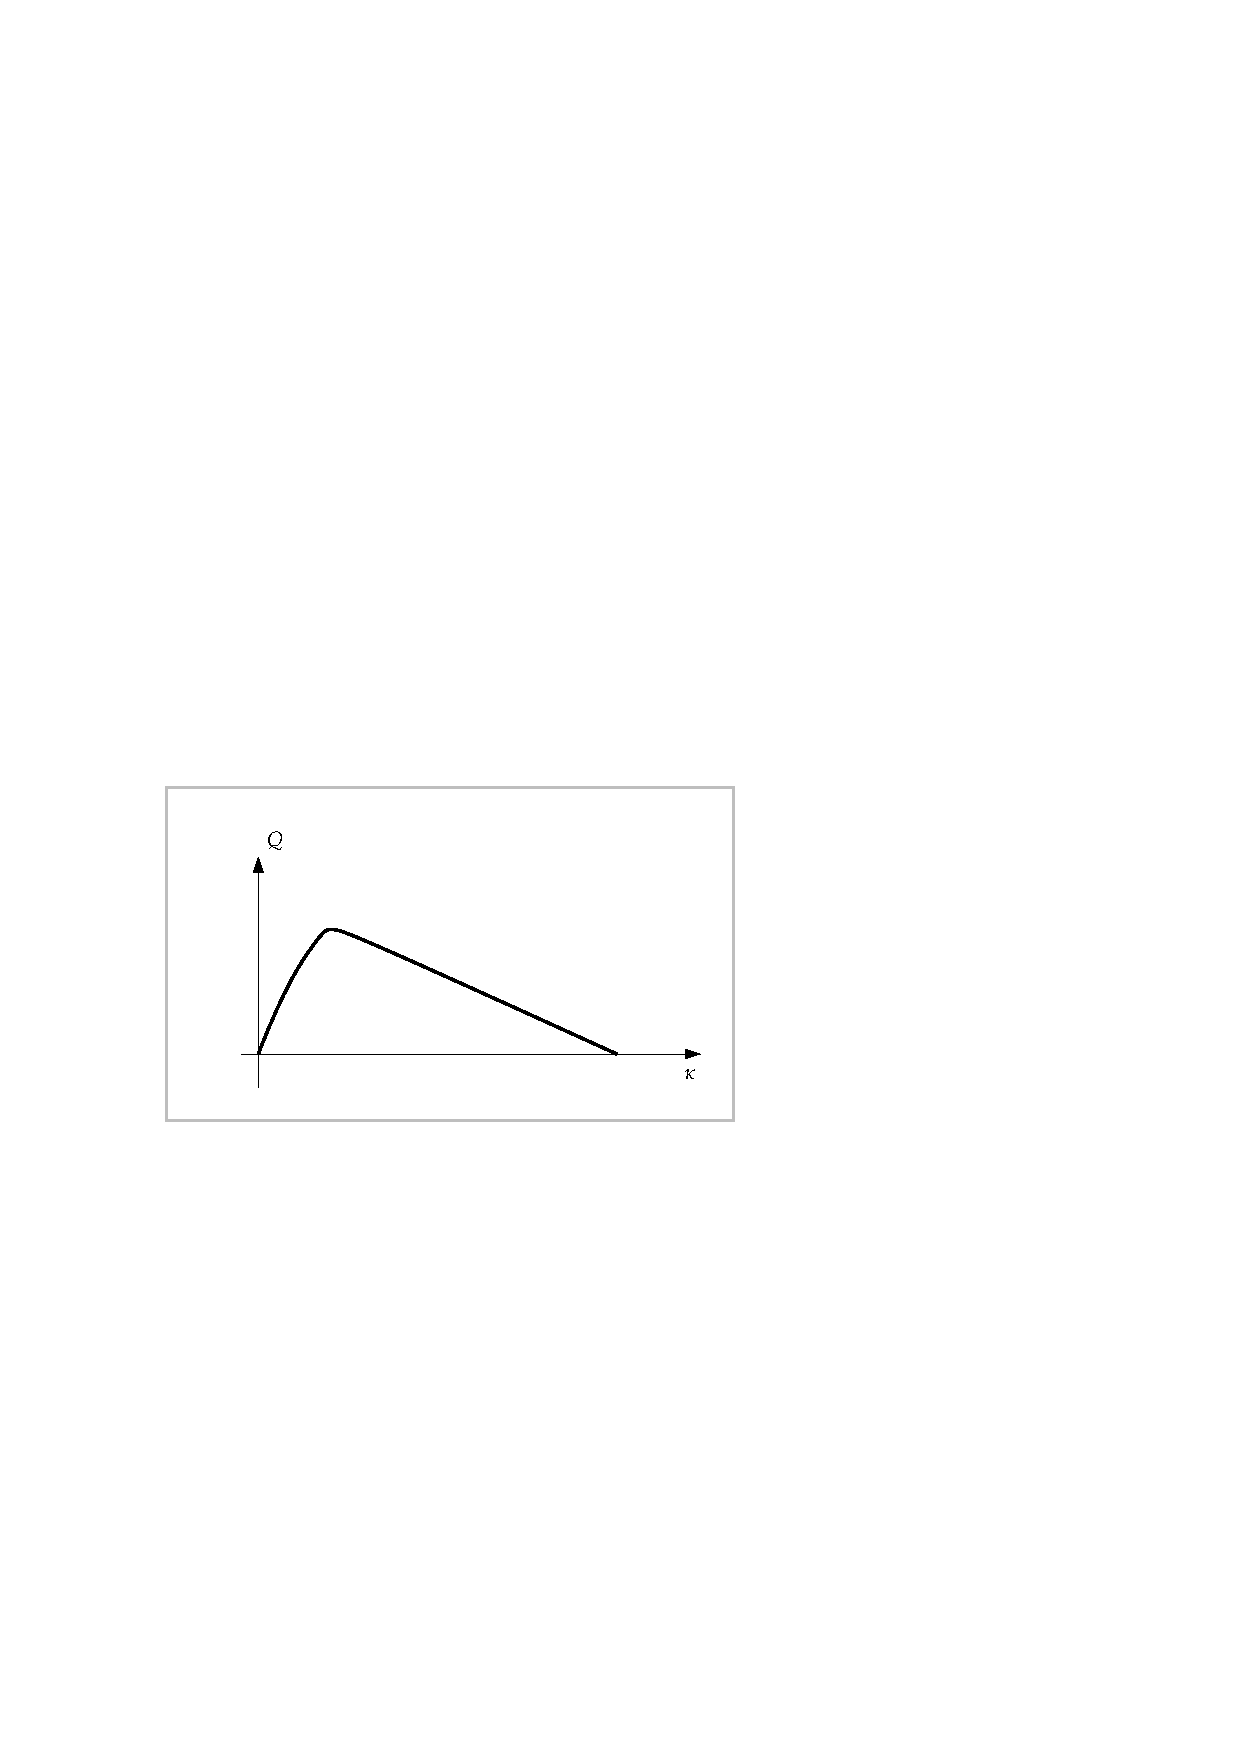
\includegraphics[width=0.6\linewidth]{fig_1a_fund_diag.pdf}\hspace*{2cm} 
      \end{figure}
      }
      \only<4|handout:0>{
      \begin{figure}
        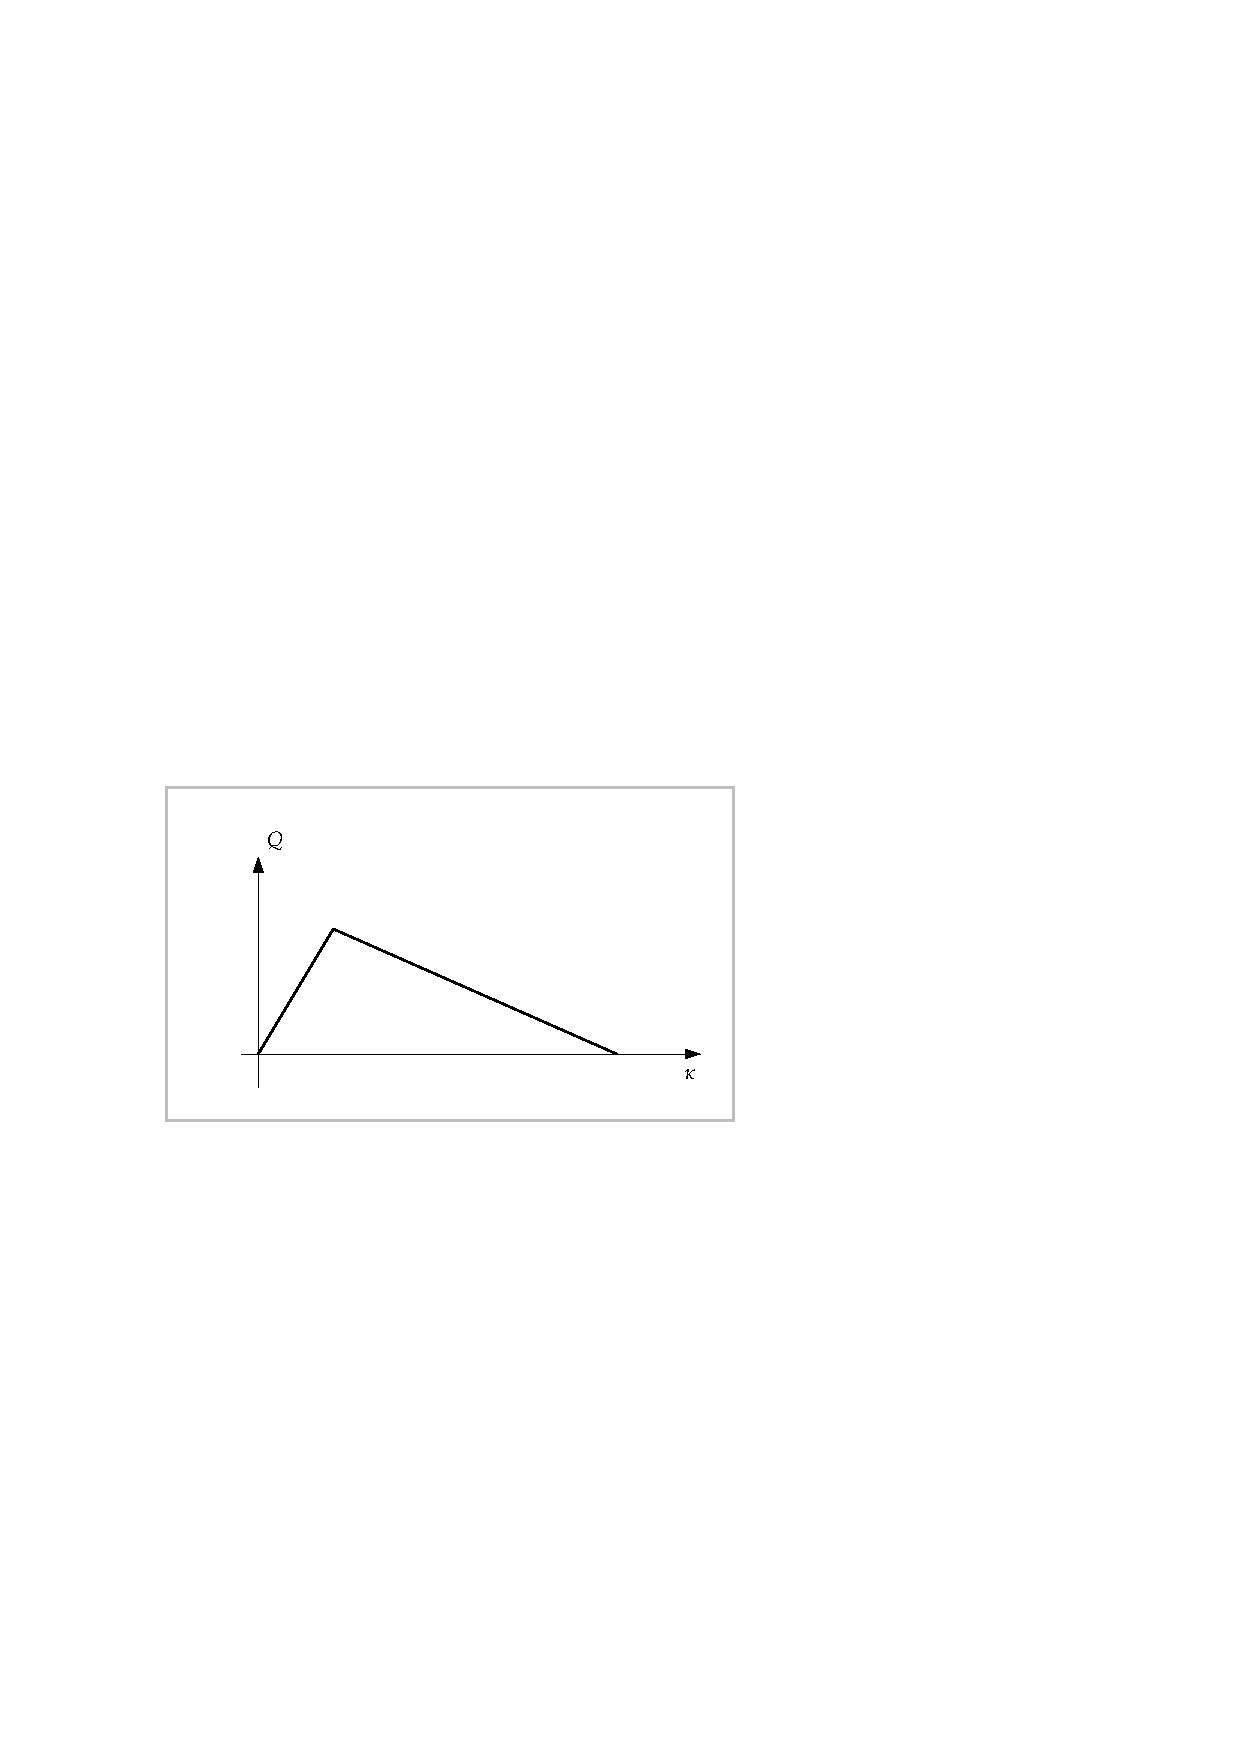
\includegraphics[width=0.6\linewidth]{fig_1b_fund_diag.pdf}\hspace*{2cm} 
      \end{figure}
      }
      \only<5|handout:0>{
      \begin{figure}
        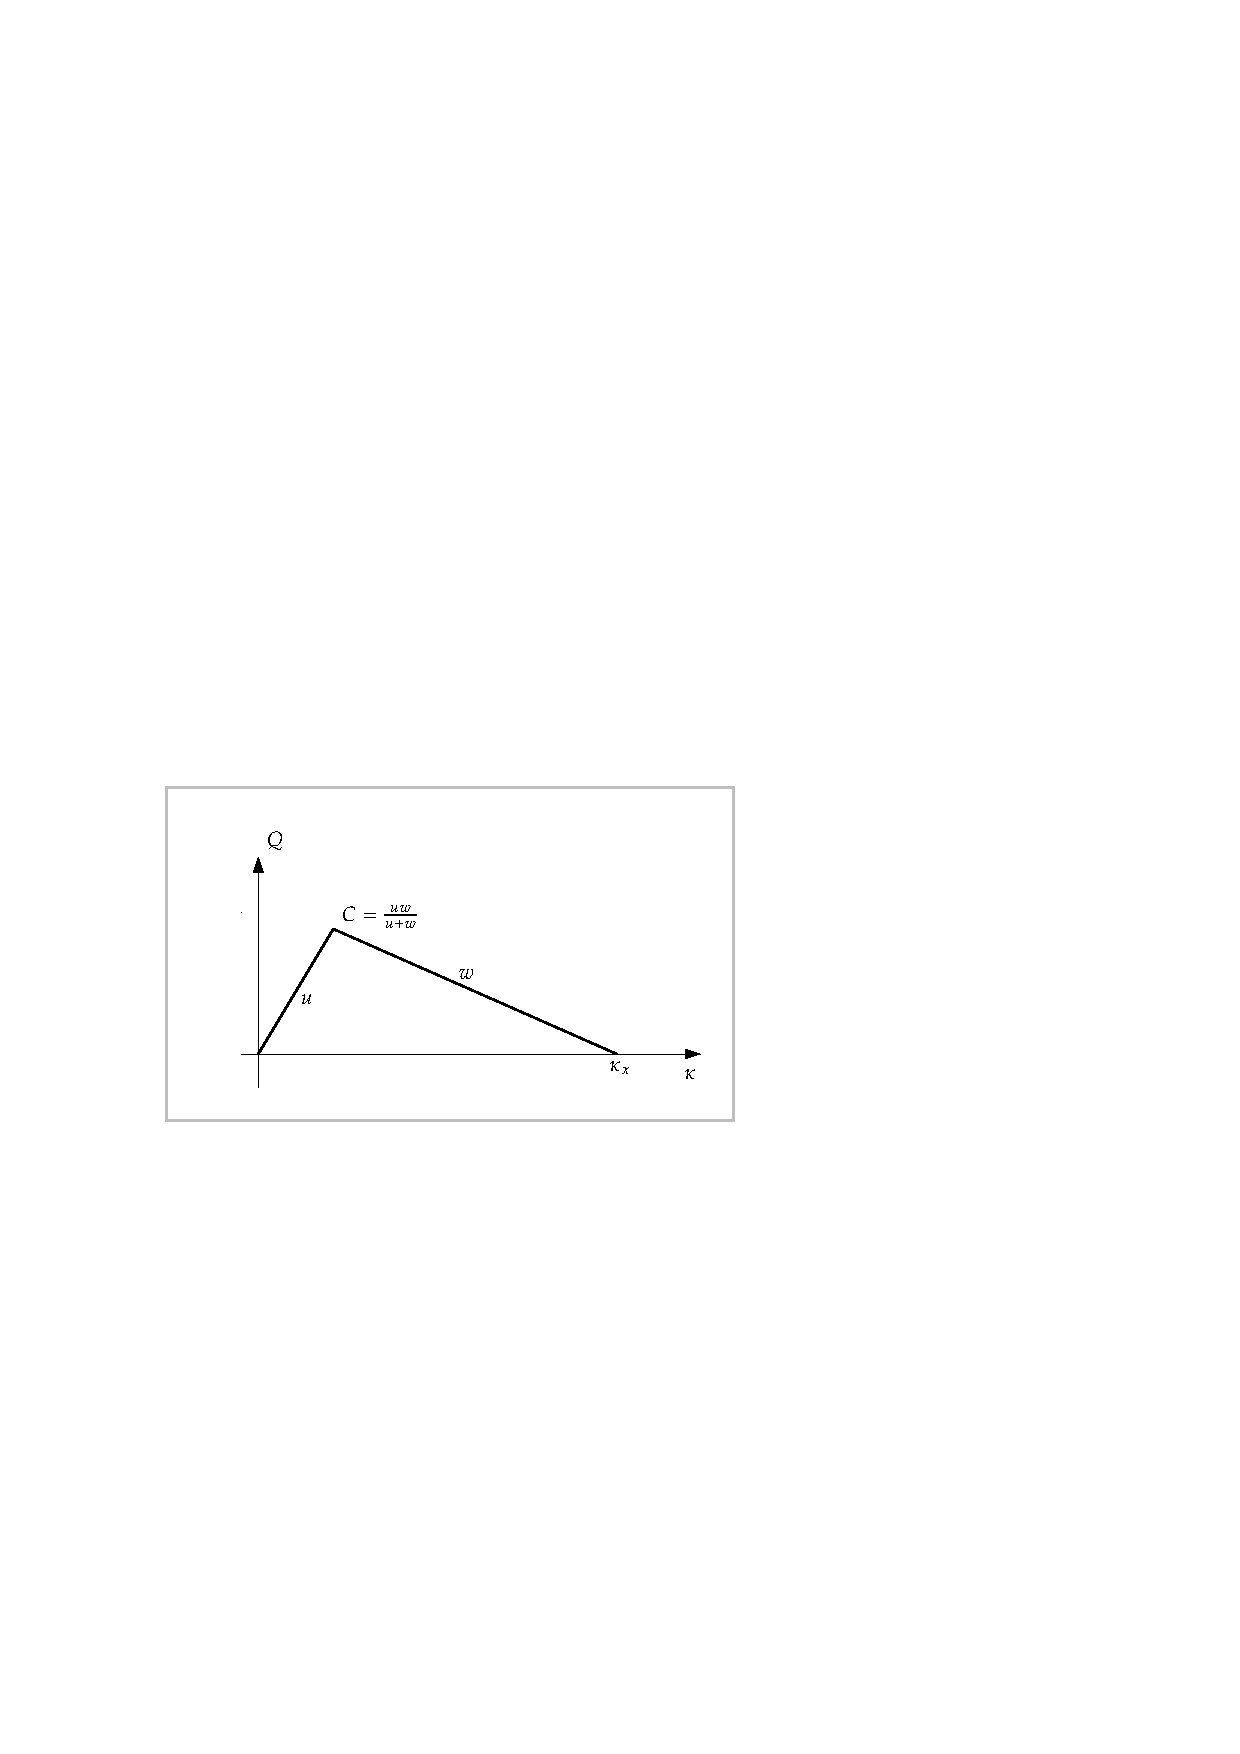
\includegraphics[width=0.6\linewidth]{fig_1c_fund_diag.pdf}\hspace*{2cm} 
      \end{figure}
      }
      \only<6|handout:1>{
      \begin{figure}
        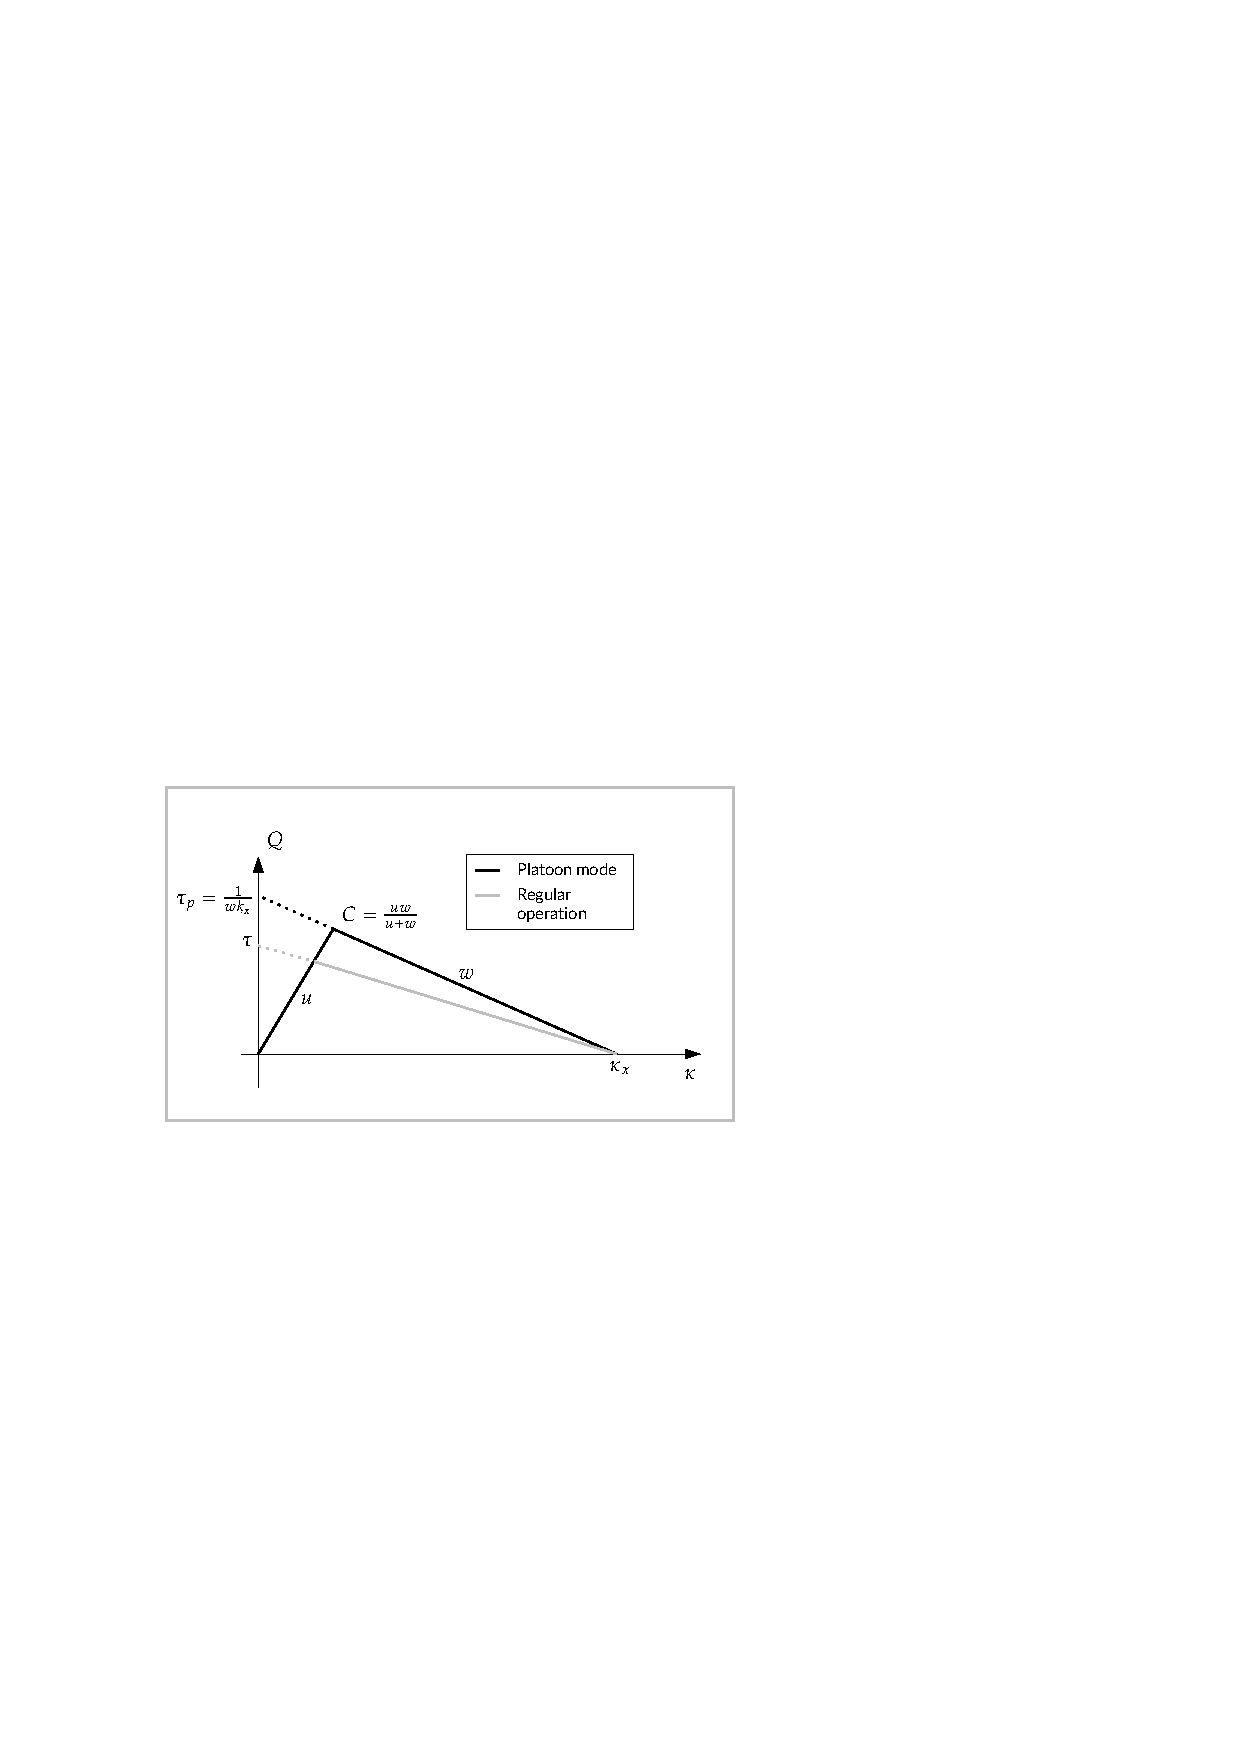
\includegraphics[width=0.6\linewidth]{fig_1d_fund_diag.pdf}\hspace*{2cm} 
      \end{figure}
      }
    \end{center}
    \end{column}
      \end{columns}
  \end{frame}